
\documentclass[twocolumn,10pt]{article}

\usepackage{times}
\usepackage{cite}
\usepackage{multirow}
\usepackage[tight,footnotesize]{subfigure}
%\usepackage{subfig}

\usepackage{url}
\usepackage{xspace}
\usepackage{amsmath}
\usepackage{amsfonts}
\usepackage{amssymb}
\usepackage{graphicx}
\newcommand{\comment}[1]{}
\newcommand{\eat}[1]{}
\usepackage{booktabs, lastpage}
\usepackage{graphicx}


\usepackage{mdframed, fancyvrb}
\usepackage[scaled]{beramono}
\definecolor{boxcolor}{gray}{0.9}
\newmdenv[linecolor=boxcolor, backgroundcolor=boxcolor, skipabove=\parsep, skipbelow=\parsep, innerleftmargin=2pt, innerrightmargin=2pt]{codeblock}

\newcommand{\myparait}[1]{\smallskip\noindent{\em {#1}:}~}
\newcommand{\myparaq}[1]{\medskip\noindent{\bf {#1}?}~}
\newcommand{\mypara}[1]{\medskip\noindent{\bf {#1}:}~}
\newcommand{\myparatight}[1]{\smallskip\noindent{\bf {#1}:}~}

\newcounter{packednmbr}
\newenvironment{packedenumerate}{\begin{list}{\thepackednmbr.}{\usecounter{packednmbr}\setlength{\itemsep}{1pt}\addtolength{\labelwidth}{-5pt}\setlength{\leftmargin}{\labelwidth}\setlength{\listparindent}{\parindent}\setlength{\parsep}{1pt}\setlength{\topsep}{3pt}}}{\end{list}}
\newenvironment{packeditemize}{\begin{list}{$\bullet$}{\setlength{\itemsep}{1pt}\addtolength{\labelwidth}{-5pt}\setlength{\leftmargin}{\labelwidth}\setlength{\listparindent}{\parindent}\setlength{\parsep}{1pt}\setlength{\topsep}{3pt}}}{\end{list}}

\usepackage{hyperref}
\hypersetup{
  colorlinks=true,      % false: boxed links; true: colored links
  linkcolor=blue,       % color of internal links
  citecolor=magenta,    % color of links to bibliography
  filecolor=cyan,       % color of file links
  urlcolor=red          % color of external links
}

\graphicspath{{./pic/}}
\definecolor{shadecolor}{gray}{0.9}

\frenchspacing
\pagestyle{plain}

\def\ala{{\`{a} la}~}
\def\ie{{i.e.}}
\def\eg{{e.g.}}
\def\etal{{et al.}~}
\def\wrt{{w.r.t.}~}
\def\viz{viz.~}
\def\vs{vs.~}
\def\etc{etc.}


\begin{document}
	\title{18731 Spring 2017 Project Report\\ IoT Device Type Identification} %of \\ Internet Routing Behavior 
	
\author{
Man Li, Qing Liu, Rongzhi Wan
  }

\maketitle

\begin{abstract}
As Internet-of-things (IoT) gets more and more popular, security issues of IoT device are gaining more attention. Device type identification is considered an important topic of IoT security for that device type can be exploited by many security approached to provide protection for IoT devices. Works have been done on extracting features from packet generated by the device and use those features for classification. This work is focused on improving classification accuracy and efficiency by applying different classifiers on different traffic types. Feature engineering techniques that can further improve performance is also explored in this work. What’s more, a real-time device type identification application with a trained classifier and a real-time traffic capture module is developed to provide users a clear view of the IoT devices in their network.
\end{abstract}


\section{Introduction}

Currently we are in the middle of the big trend of IoT (Internet-of-things). Connecting identifiable smart devices allowing them to exchange data has facilitated people’s life greatly. The number of IoT devices is estimated to reach 24 billion in 2020 \cite{greenough_2016_website}. Because of various reasons such as lack of security considerations in the initial device design phase, support no longer available for old devices, or limited computing power in the device, it is unrealistic to expect every IoT device to be installed with security frameworks. Thus, central controllers that are responsible for securing connections among IoT devices and connections between IoT devices and the Internet are needed. One important feature in such controllers is the ability to classify IoT devices based on its traffic. This feature can help detect unauthorized IoT devices \cite{meidan_2017_unauthorized}, provide different device type with different isolation level \cite{miettinen2017iot}, and so on.

Our project focused on IoT device type identification. We trained a classifier that combines random forest classifier and edit distance to analyze the device type from the traffic during the setup period of each device. We wrote a demo program that captures traffic and performs the classification in real time.

\section{Related Work}

Many works on IoT devices identification have been done. One of them is ”IoT SENTINEL” \cite{miettinen2017iot}. This system is able to automatically identify the types of devices being connected to an IoT network, and to enable corresponding enforcement rules. This system is based on passively observed network traffic during the setup phase of smart home devices. After fingerprinting, devices can be classified by comparing the edit distance of their fingerprints.

Another related work is an analysis of Home IoT network traffic and behaviour \cite{amar2018analysis} . In the setting a smart home, this work aims to understand the overall IO behaviour of devices, including protocol used, data volumes, type, data rate and transmission frequency, etc. Different from IoT SENTINEL, this analysis is based on a relatively long term traffic, including both setup phase and further communications. Also, different from IoT SENTINEL who adopts machine learning techniques, this work uses statistics-based analysis.

These works provide valuable insights and outcomes, yet there are some improvements can be done to better identify devices. One of them is feature selection: in IoT SENTINEL, 23 features are chosen, including the type of protocols used across different layers, packet header information, packet size and so on. In the analysis of home IoT network, it has chosen many features in common such as protocols and data volumes. It also selects different features like data rate and transmission frequency. In our work, in the setting of smart home, we will select more representative and distinguishable features based on a series of experiments. This is expected to yield a higher classification rate. In addition, this work also will focus on the study of unauthorized device identification. In both of those works mentioned above, device type is defined as manufacture plus device model. Here we try to produce a more general device type for unseen manufacture.

Another contribution of this work is to develop a real time IoT device type application for user to monitor the IoT device connection status in their network. We hope to develop a framework that utilize the trained classifier and capture traffic to produce classification result for device newly connects to the network in real time. This framework can be the foundation for many extensional functions, like device white/black list, device connection management customized user notification and suspicious device alerts.




\section{Approach and Project Description}

Figure \ref{fig: system overveiw} shows the overall structure of our system. Traffic in the network is captured and processed to generate fingerprints. Then fingerprints are fed into classifier  for either training or testing. During testing, classification results are displayed at a monitoring page. All the code and data can be accessed in our git repo \href{https://github.com/RongzhiWan/18731project}{here}. 

This section is organized in the following way. First we discuss problems in fingerprints generation, including traffic capturing and feature extraction. Then the classifiers used in this system will be covered in detail. We also give a simple solution for unauthorized device identification in this section. Lastly, the demo application and the complete work flow is introduced to give a general view about how the whole system work.



\begin{figure}[h]
  \centering
   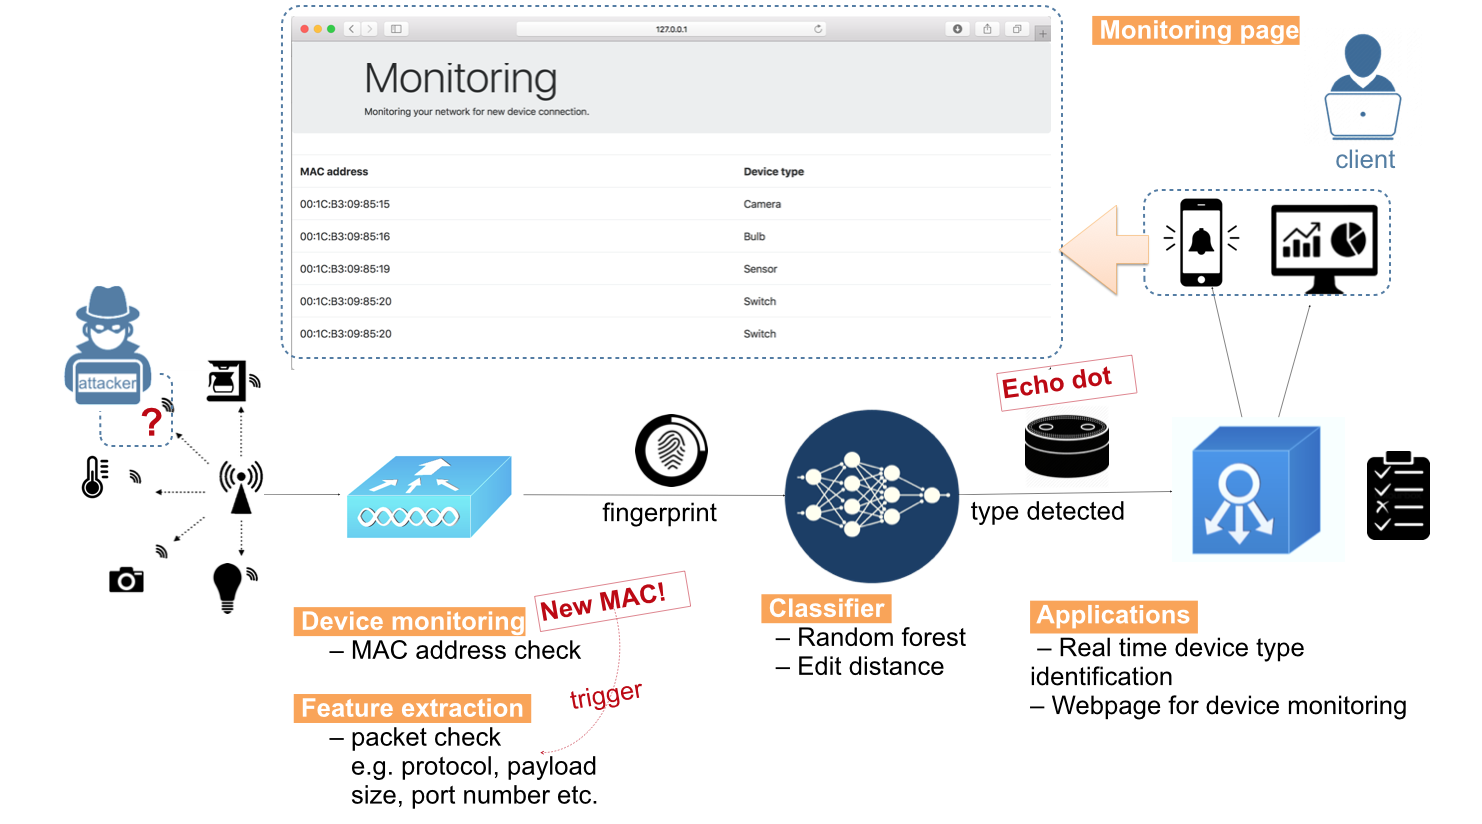
\includegraphics[scale=0.3]{system_diagram}
  \caption[System overview]{System overview.}
  \label{fig: system overveiw}
\end{figure}


\subsection{Fingerprint generation}

To generate fingerprints, the first step is to capture traffic from the network, then the next step is to extract features from the captured traffic packets and features for a sequence of packets will be used to generate one fingerprint.

\subsubsection{Traffic capture}

There are many options to capture IoT device traffic. In terms of how capturing tools interact with IoT devices, there are passive approach and active approach \cite{free_hacking_articles}.

\textbf{Passive sniffing} Passive approach employs packet sniffing tools such as Wireshark, tcpdump, Capsa and so on. Those tools don not actively send traffic to devices. Passive sniffing usually cannot be detected.

\textbf{Active sniffing}  Active sniffing requires a sniffer actively send traffic to devices, then captures subsequent traffic from devices. Such traffic can be ARP spoofing, traffic floods and so on. Active sniffing is detectable by most devices.
\newline
\newline
In terms of device and environment setup, there are simulation/emulation approach and experiment approach.

\textbf{Simulation}
A simulated environment does not require the presence of physical devices. There are many simulation tools available, such as IBM Bluemix \cite{edprosser_2016} and IoTIFY \cite{rapid_iot_application_development}. Simulation tools and platforms focus on the behaviors of devices. Many of them use virtualization technologies, so actual network traffic is usually modified or hidden.

\textbf{Emulation}
An emulated environment duplicates the inner workings of devices, but do not necessarily require the presence of physical devices. One IoT firmware emulation tool is Attify \cite{attify_iot_and_mobile_security}. The biggest challenge of using firmware emulation is to get firmware of variant types of IoT devices and keep it up-to-date. Some manufacturers do not make their firmware public. For those public firmware, many of them is not up to date.

\textbf{Experiment with real devices}
An experimental environment requires the presence of physical devices. This approach provides traffic more similar to the actual use cases. The biggest challenge of setting up environment with real devices is the shortage of devices and manual setup. For example, to set up an Amazon Echo dot, we need to download mobile application and follow several steps such Wi-Fi selection, pressing button.
\newline
\newline
In terms of duration of capturing, there are short-time approach and long-time approach.

\textbf{Short-time}
Short-time approach tries to capture traffic in a short duration. The selected duration can be special period, such as initialization time, busy communication period, shut-off period and so on. Behaviors in different periods usually vary from each other.

\textbf{Long-term}
Long-term approach keeps track of traffic for a relatively longer period. For example, \cite{amar2018analysis} captures traffic for 22 days continuously. This provides adequate data but requires more filtering and analyzing.

In this project, we use passive sniffer to capture real device traffic during setup period. Using passive sniffer is out of security concern. IoT device identification is intended to be used for network controllers, secure gateway, monitoring system and other applications, so we don’t want it to be detectable. Using real devices provides us with realistic data. All devices need to setup before they proceed to actual use, and such phase is controlled by firmware, usually not configurable by customers. Therefore, we decided to capture data during setup phase to prevent malicious attackers from launching traffic floods to fool the classifier.

As shown in the system diagram in Figure ~\ref{fig: system overveiw}, devices are connected to the hotspot. Packet sniffer Wireshark is running on the computer who launches the hotspot, so that all traffic via hotspot will be captured. Due to limit of available devices, we employed some data from \cite{miettinen2017iot}. Table ~\ref{tab: dev} shows a full list of devices used in this project.



\begin{table}[]
\centering
\scriptsize
\begin{tabular}{llll}
\textbf{Number} & \textbf{Device}                     & \textbf{Type by function} & \textbf{Manufacturer} \\
1      & Aria                       & scale            & Fitbit       \\
2      & DCH-935L                   & camera           & D-Link       \\
3      & DCS-930L                   & camera           & D-Link       \\
4      & D-Link sensor           & sensor (window \& door) & D-Link       \\
5      & DCH-G020                   & home hub         & D-Link       \\
6      & DCH-S150                   & sensor (motion)  & D-Link       \\
7      & DCH-S220                   & siren            & D-Link       \\
8      & DCH-S160                   & sensor (water)   & D-Link       \\
9      & IC-3115W                   & camera           & Edimax       \\
10     & SP-1101W                   & plug             & Edimax       \\
11     & SP-2101W                   & plug             & Edimax       \\
12     & Cube MJPEG                 & camera           & Ednet        \\
13     & Ednet.living               & gateway          & Ednet        \\
14     & HMIP-PS                    & switch           & Homematic    \\
15     & Hue 3241312018             & light bridge     & Philips      \\
16     & Hue PTM 215Z               & light switch     & Philips      \\
17     & SMK20-EU                   & kettle           & Smarter      \\
18     & SMC10-EU                   & coffee machine   & Smarter      \\
19     & Lightify                   & gateway          & Osram        \\
20     & BC-LGW-O-TW                & gateway          & eQ-3         \\
21     & LB100                      & bulb             & TP-Link      \\
22     & HS100                      & plug             & TP-Link      \\
23     & HS110                      & plug             & TP-Link      \\
24     & F7C029de                   & plug             & WeMo         \\
25     & F7C031vf                   & light bridge     & WeMo         \\
26     & F7C027de                   & switch           & WeMo         \\
27     & WS-30                      & scale            & Withings     \\
28     & Echo dot                   & voice assistant  & Amazon       \\
29     & Google Home mini           & voice assistant  & Google       \\
30     & Powerstrip01               & plug             & Tonbux      
\end{tabular}
\caption{Devices used in experiments of this project.}
\label{tab: dev}
\end{table}


\subsubsection{Feature extraction}

Different IoT device types use different protocols, have different communication sequences, and send packets with different sizes. Such features is the key to differentiate them. In feature extraction phase, we focus on these features:

\begin{enumerate}
  \item Protocol features
  \begin{itemize}
  \item Link layer protocol: ARP / LLC
  \item Network layer protocol: IP / ICMP / ICMPv6 / EAPoL
  \item Transport layer protocol: TCP / UDP
  \item Application layer protocol: HTTP / TLS/SSL / DHCP / BOOTP / SSDP / DNS / MDNS / NTP / MQTT / IGMP / TFTP / QUIC / STUN
  \end{itemize}
  \item Network layer features
  \begin{itemize}
  \item IP options: Padding / RouterAlert
  \item Packet content:  Packet size / Raw data size
  \item IP address: Source IP address / Destination IP address 
  \end{itemize}
  \item Transport layer features
  \begin{itemize}
  \item Port class: Source port number / Destination port number
  \end{itemize}
\end{enumerate}

To extract features from captured raw data, we wrote a Python script using "dpkt" package. Output of feature extraction is $m$ files, each of them contains $k$ lines whose format is presented below. Each fingerprint is represented as a $f*n$ matrix {\bf F}. To prepare for the classification phase, we define our training data as the following format.

{\bf type\_number\quad F\_row\_cnt \quad F\_col\_cnt \quad flattened\_F}

Note that $f$ is number of features and $f$ is 29 in our experiment. $n$ is the number of packets in each capture. $m$ is the number of devices. $k$ is number of captures for a device. In our case, most of $k$ is 20.


\subsection{Classifiers}

After fingerprints from each packet in the device setup phase are extracted, the data is passed into classification. Our classifier is consist of two layers of classifiers. The first layer is a random forest classifier and the second layer is an edit distance classifier. 

\subsubsection{Random forest}

In the first stage of the classifier, a binary random forest classifier is used. The input to the classifier for each device setup capture is features from up to the first N packets concatenated together. If some device setup has less than N packets, zeros are padded.

A binary classifier is used for each device type so that our model is more scalable. If a single random forest classifier is used, in the case that there are a lot of device types and a lot of training examples, reloading the whole forest might take too long. With a binary classifier for each device type, we would only need to train a new classifier when a new device type is added. Also, if a device’s software is updated and the packets it send during the setup phase are change, we need to only re-train that single binary classifier for that device, rather than the whole classifier.

Random forest classifier is chosen because the algorithm doesn’t need much prior feature selection. We can use all the available features and the classifier will select the important features for us. We tried using FSM (finite state machine) to classify whether a capture might belongs to some device. However, we found that because the features we selected are too specific, there is a difference between the states learnt by the FSM during training and the states FSM sees during testing, and thus, no packet fingerprint in the testing data appears in the training data.

The output of this first stage for each device setup capture is an array that represents the possibility this device belong to any of the device types. The output data can be used to predict the device type by finding the type with the highest confidence, or can be used as data assist with the second stage of our classifier, the edit distance classifier.

We don’t have a seperate testing dataset. To test the accuracy of our model on this layer, we separate the training data into several folds (10 in the result described below) and cross validate our model. When we wrote the demo, all the training data are used to train our model so that the model can be more accurate during real time classification. 


\subsubsection{Edit distance}

Random Forest Classifier produces a candidate list for a device. The second layer of classifier, Edit distance classifier, will select the final device type from this candidate list. To calculate edit distance for fingerprints, we need to represent fingerprint as a word. Recall that each column in a fingerprint is representing a packet. By assigning a distinct ID for each packet(column), will be able to represent a fingerprint in a word-like manner. A fingerprint with n columns will be represented as a word with n characters. 

After having word representation for each fingerprint, we can calculate a dissimilarity score for the testing fingerprint with all potential candidate device types. For each candidate device type, 5 fingerprints are randomly sampled as group truth. Edit distance is calculated using Damerau-Levenshtein edit distance algorithm between testing fingerprint and 5 sampled scores. The 5 scores are normalized by dividing the longest distance. Those 5 scores are summed up to calculate the final score for this testing fingerprint with current device type. After calculating a score for all candidates, the device type with smallest dissimilarity score will be chosen as final device type. 

\subsection{Unauthorized devices identification}

Another goal of this work is to identify unauthorized devices. From our experiments, we found that it’s generally difficult to train a classifier that can identify a certain device type from different manufactures. The reason is that the protocol design is highly diverse across different manufactures. On the other hand, different devices from the same manufacture tend to have similar traffic pattern. Those two problems make the task of  training a classifier that classifies same device type across different manufactures challenging. If we imagining represent all the fingerprints we learned in the same vector space, fingerprints of the same device type but different manufactures will be far away form each other because the sequences and number of packets will be very different for those fingerprints. While different device types from the same manufacture will have fingerprints close to each other. As a result,  a classifier capable of classifying the same device type across different manufactures as one category will have a high confusion rate among device type from the same manufacture. 

Bases on the above discussion, we consider there are two challenge in the identification of unauthorized devices. The first is to identify same device type from different manufactures. The second is identify different device types from the same manufacture. To balance the accuracy between those two types of classification task, the method we used here is to first classify devices in fine granularity (identify different device types from the same manufacture)  then cluster the specific categories we obtained (D-LinkCam, EdimaxCam2, D-LinkSwitch, WemoSwitch) into more general categories (camera, switch). 

The most simple approach to map the specific category to general category is to manually configure a list of specific device type for each general decide type. The specific device type is defined as device type plus manufacture while general decide type is defined as device type and no manufacture. Therefore the list will be like: “camera” : [“D-LinkCam”, “EdimaxCam2”], “switch” : [“D-LinkSwitch”,”WemoSwitch”]. 

In short, our current solution for unauthorized device identification is to first train a classifier for specific device type (device type plus manufacture) then use the mapping list to assign a general decide type. To make this approach works in scenario involving diverse device types and manufactures, the model need to be trained on training data with a sufficient coverage on mainstream manufactures’ device traffic. If a large dataset can be built to collect the device traffic of mainstream IoT manufactures, it can be very helpful for not only  unauthorized device identification but also simplify IoT device identification in an environment without large amount of data traffic, otherwise it may take a considerable amount of time to collect enough data for training a classifier.

\subsection{Real-time IoT device type identification application}

This work also aims at providing an application interface where user can monitor the new IoT device connection and manage those connections of IoT devices in the network. In this work, we developed a real time IoT device identification application. 

The application is consist of three parts:  a real time packets capture module that is capable of generating fingerprints from traffic within the network, a trained classifier that identify device type based on the fingerprint and a webpage that showing a list of IoT devices currently connected to the network. A complete work flow is shown in Figure ~\ref{fig: demo}.

\begin{figure}[h]
  \centering
   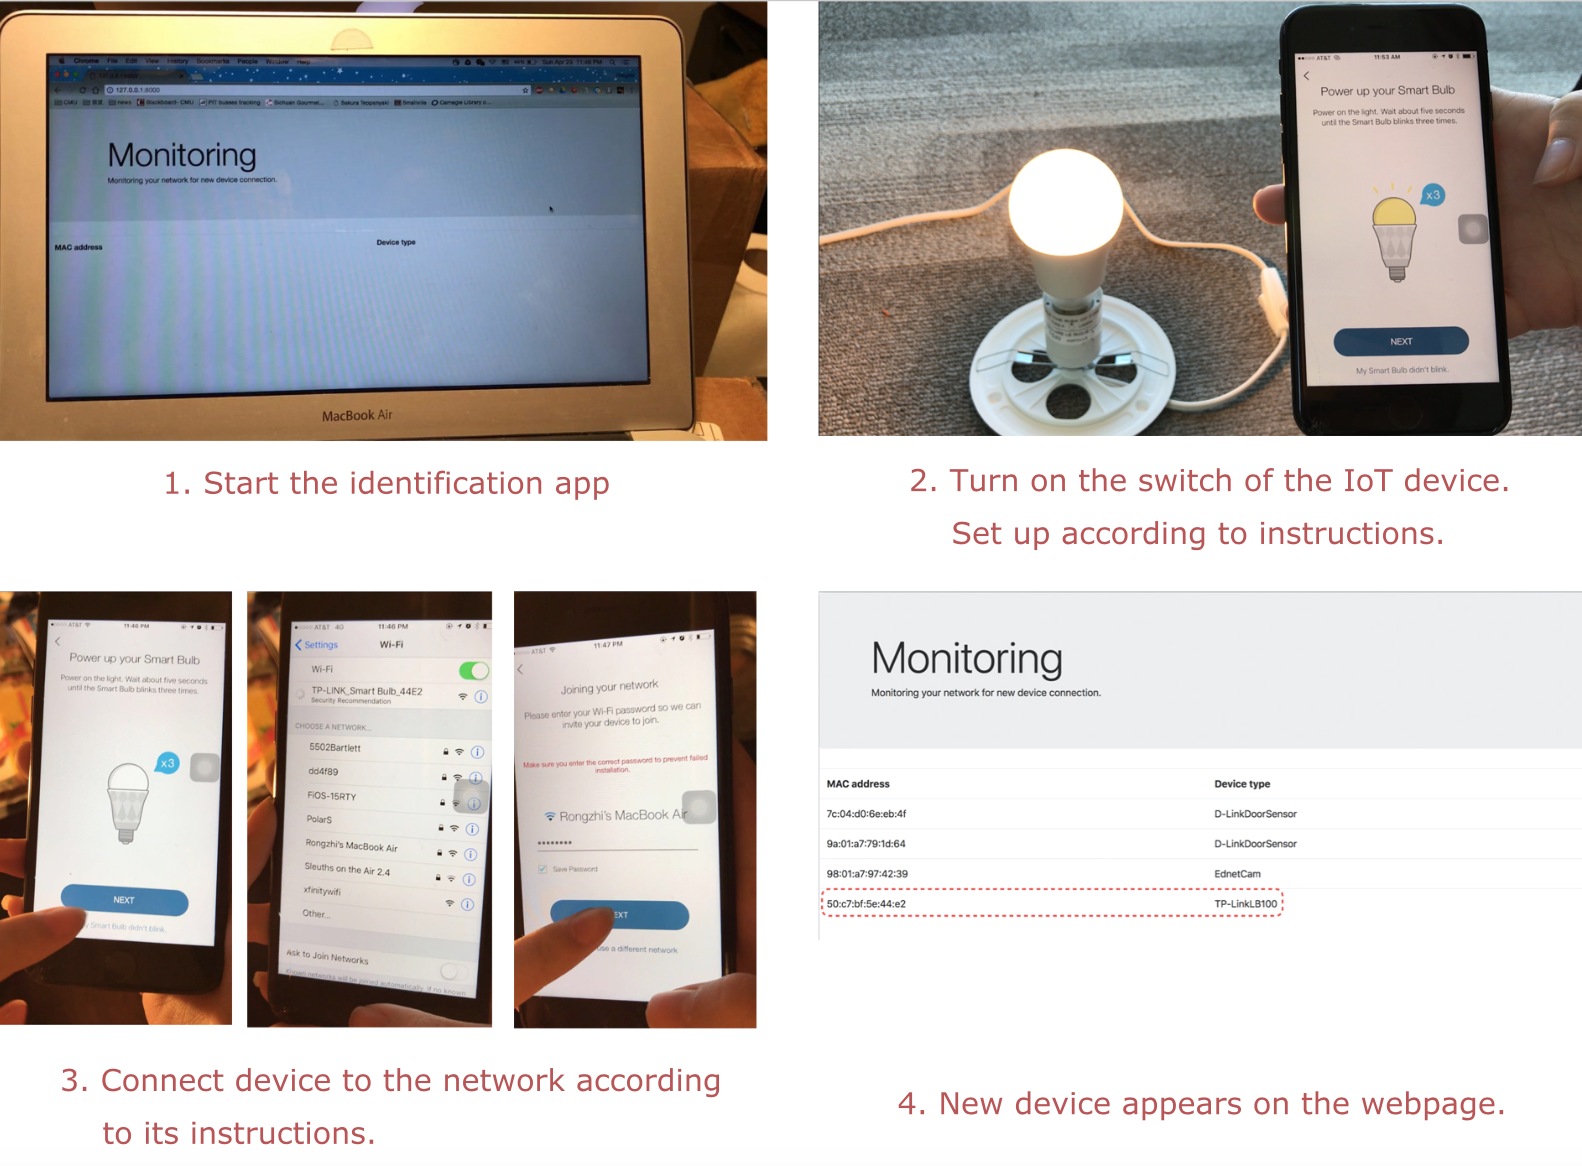
\includegraphics[scale=0.29]{demo}
  \caption[Work flow for the real-time IoT device type identification application]{Work flow for the real-time IoT device type identification application.}
  \label{fig: demo}
\end{figure}

Currently this application is only a prototype for demo purpose with many limitations. But we’ve planned out many interesting functions that can be supported by extending the current version. For example, to packets for analyzing purpose, the laptop running the program needs to provide hot-spot connection to the IoT devices. We hope to extend this to allow the laptop to use monitor mode to capture packets from IoT devices in the same VLAN. Another function we want to support is device connection management. Currently it’s only showing the device list. We hope this can be extended to an interface where user can manage the device network connection of IoT devices by interacting on the webpage. Other functions like “sensitive derive list” are also expected. User can set a list of sensitive devices like camera or sensor. Once connection attempt of such device types is detected, the use will be informed with a text message or email. 


\section{Challenges and problems}
In this section, we summarize the challenges we encountered during our work on this project. Those can be generally existing problems in similar IoT device identification studies, therefore we hope to provide a foresight for potential challenges in experiment process and system design to help future IoT device studies better prepared.

\subsection{Setup environment}

As aforementioned, there are three options to capture device traffic: simulation, emulation, and using real devices. In this project to obtain traffic more like real cases, we chose to setup environment for capturing real device traffic, and this is the first challenge.

\textbf{Sniffing interface} To use a packet sniffer, we setup a hotspot on computer and run Wireshark on it. Devices are connected with the computer via wireless Wi-Fi interface, and the computer is connected with Ethernet via Ethernet cable interface. A packet sniffer will capture traffic on Wi-Fi interface. However, Wireshark on a Linux machine is unable to interpret traffic via Wi-Fi interface from link layer to higher layer. To solve this problem, we tried different machines and found Wireshark on MacOS can successfully interpret Wi-Fi interface traffic on all levels.

\textbf{Manually setup} Many devices require manual setup. One example is TP-Link LB100 smart bulb. To setup, we need to download a mobile application developed by TP-Link, connect bulb, press button in a certain button, and follow other instructions. One time of setup takes about 120 seconds, and we need to repeat such process for ten to twenty times to get multiple batches of capture.

\textbf{Shortage of device} Due to limit of devices, we employed data from \cite{miettinen2017iot}. We successfully captured data of the following devices: Amazon Echo dot, Google Home mini, Tonbux powerstrip (smart plug), TP-LinkLB100 (smart bulb).

\subsection{Environment-dependent traffic}

A new challenge followed by obtaining traffic data from different sources is that some of the devices have environment-dependent behavior. For example, a smart bulb connecting with an Apple laptop may have different ARP and EAPoL traffic from connecting with a Dell computer running Redhat due to different hardware and operating system of the hotspot host. To rule out this effect, we use Edit Distance classifier to better identify those devices from the same manufacturers. More details can be found in Conclusion section.

\subsection{Whitelist}

After we have captured multiple setup traffic of multiple devices for training, we need to consider how to capture traffic in a real time monitoring system.
 
Before traffic is analyzed, a rough way to identify a device is to examine its MAC address. In real time monitoring system, this can be a signal to start capturing traffic for this new device in LAN. One problem is that there are many background processes running on hotspot host. So we let the host run for some time and record seen MAC addresses. When there is no new MAC address being added on the list, we can get a list of “white” MAC addresses. For further traffic monitoring, these MAC addresses will not be considered to be new devices.
 
One thing to notice is that MAC address can be spoofed. So relying on MAC address to identify a device, or relying on getting manufacturer information from MAC address fields is not safe. How to prevent from being fooled by MAC address spoofing and how to find a better signal to start capturing traffic is considered as future work.


\section{Results}

\subsection{Classifier experiments}

In this we experimented with different combinations of classifiers. Currently there are two layers of classifiers: random forest and edit distance. The first layer classifier, random forest can be also used along without the second layer for that it can give a real number probability for each device type besides giving a binary value each device type. In a “two layer classier” setting, we are using the binary output of random forest classifier. But if we use the probability output of random forest classifier, we’ll be able to select the most possible device type by choosing the one with highest possibility. In this way, only one layer classifier is needed.

We tested the “One layer classifier” and “Two layer classifier” separately, and got the result shown in Figure ~\ref{fig: res1}.


\begin{figure}[h]
  \centering
   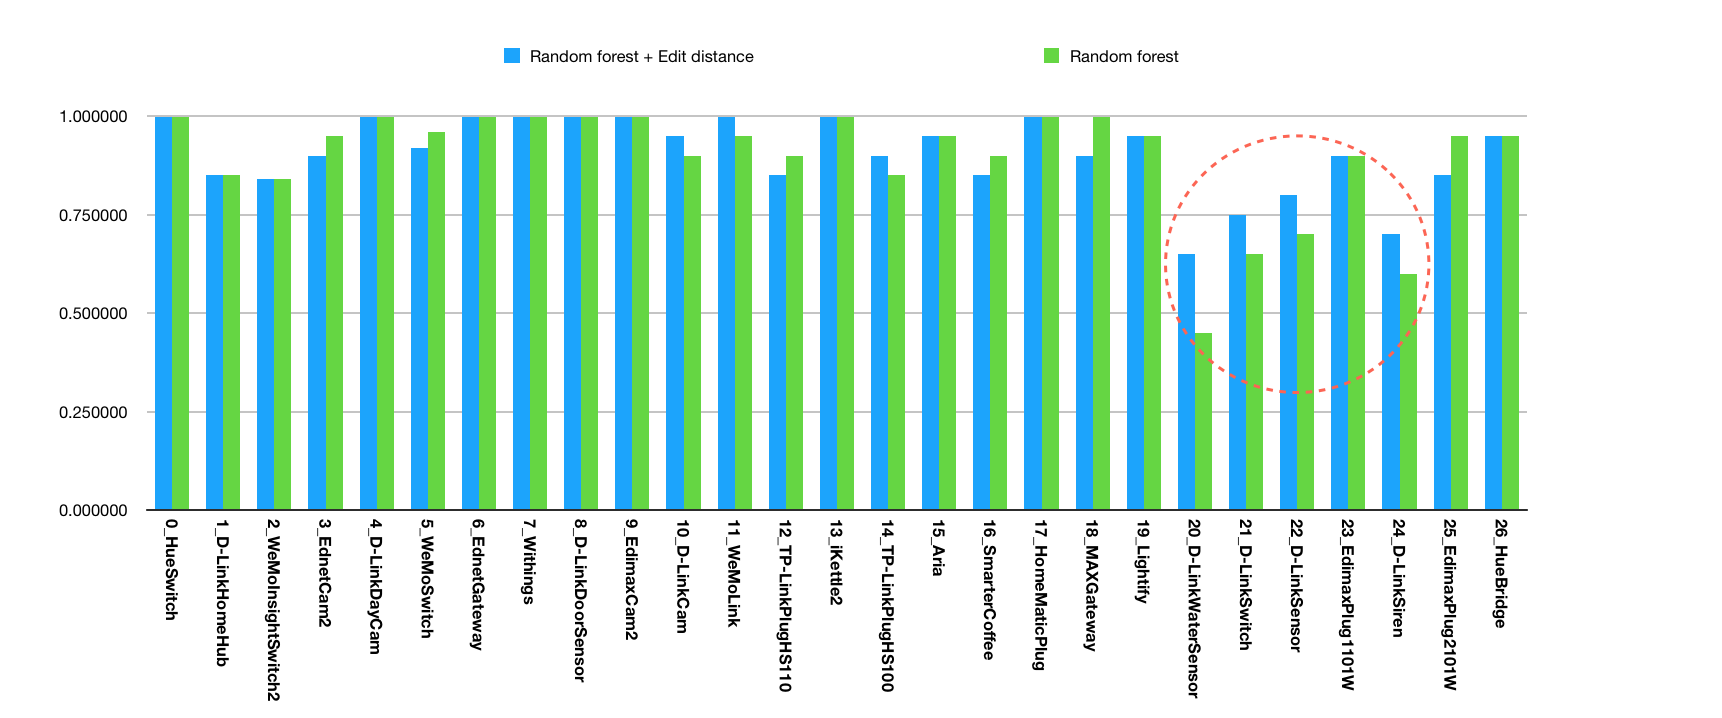
\includegraphics[scale=0.3]{res1}
  \caption{Performance for each device type with one layer classifier and two layers classifiers.}
  \label{fig: res1}
\end{figure}

One interesting finding from the experiment result is that in most of the cases, random forest classifier works better or as good as two layers of classifiers. This indicates that generally speaking, when there are multiple type candidates, using the probability output of random forest classifier is better than using its binary output and using edit distance to select the best candidate. However, there is an exception where random forest doesn’t work well by itself and a second layer classifier actually improve the performance. This is the classification for devices made by the same manufacture. As discussed in the previous section, devices from the same manufacture tend to share very similar traffic pattern due to the fact that they may be using the same protocol design. Therefore for those devices, they are more likely to be misclassified by the random forest classifier. Introduction of second layer classifier can help with this scenario for that the edit distance classifier used in the second layer provides are more refined classification result based on the output of random forest classifier. 

\subsection{Feature engineering experiments}

Devices are identified by analyzing their traffic, more specifically, the packet contents and sequence. Therefore, how to choose features has a deterministic effect. After a series of experiments, we have the following findings.

\textbf{Number of features}
It is expected that the more features we capture, the better we can differentiate devices. Our experiments certified this. As Figure ~\ref{fig: res2} shows, adding more features yields a higher classification accuracy for part of the devices while other devices may have a lower classification accuracy. However, what's worth noticing is that there are more device types improved by adding more features than the ones whose accuracy is decreased.

\begin{figure}[h]
  \centering
   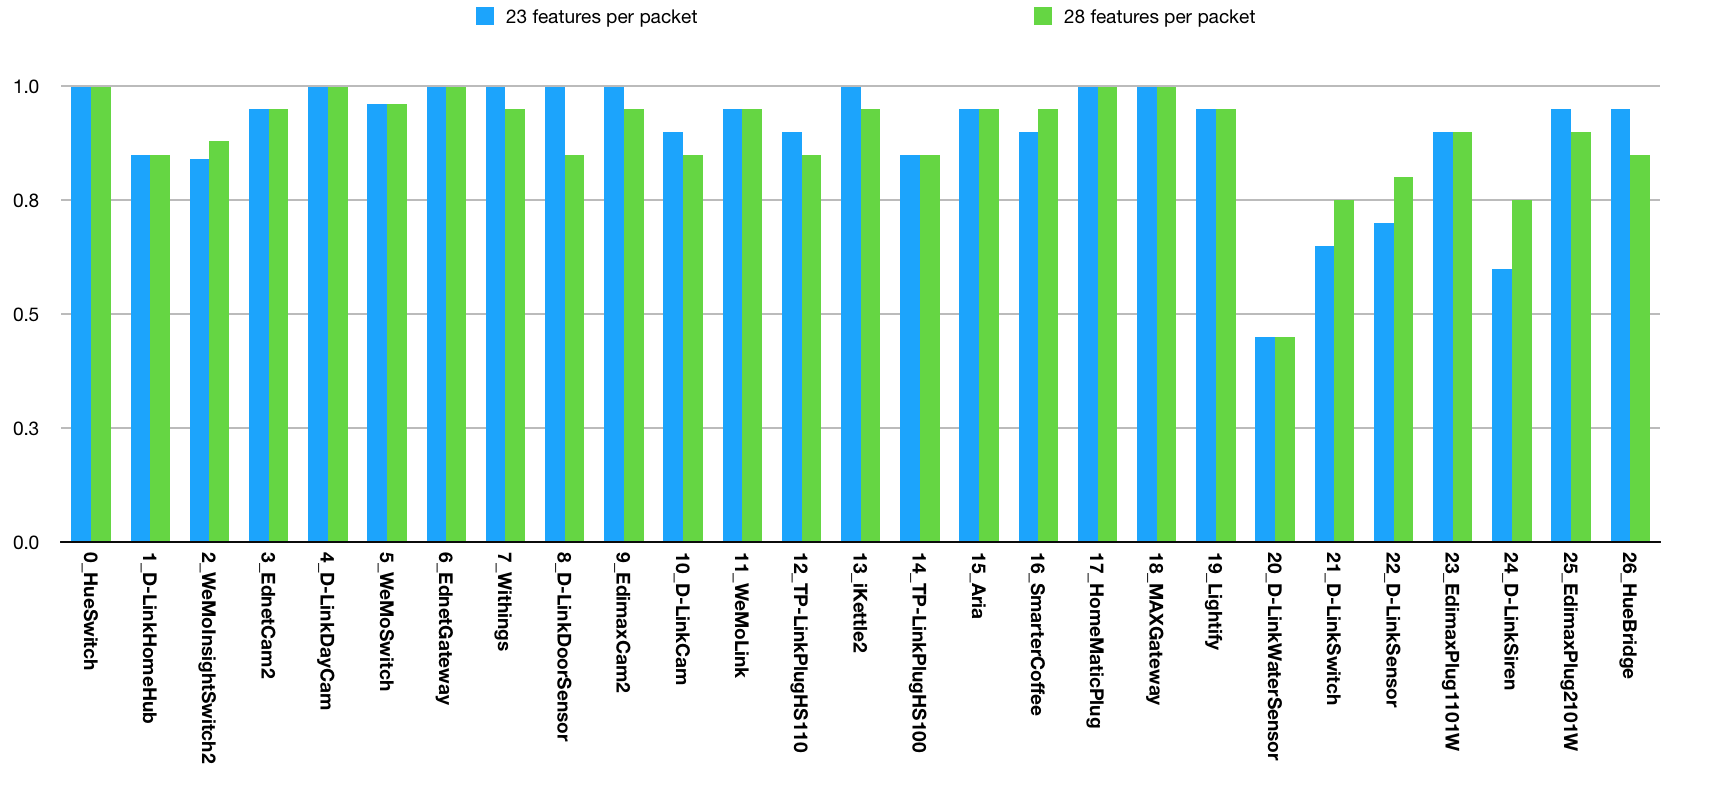
\includegraphics[scale=0.28]{res2}
  \caption{Performance for less features and more feature used.}
  \label{fig: res2}
\end{figure}

\textbf{Deterministic features for devices by same manufacturer}
Devices from same manufacturer usually have very similar traffic. This may because manufacturers have their own logic and process to setup a device. These devices are likely to have similar sequence of packets of different protocols, packet size, number of packets and so on. Therefore, we need some deterministic features to differentiate them. One of the features is source and destination IP addresses. As Figure \ref{fig: res3} shows, with source and destination IP address feature, the classification accuracy is higher than without this feature. This is not difficult to understand, because in a same LAN, devices are usually assigned with different IP addresses. Even though they have very similar traffic pattern, they need to be differentiable from network communication perspective.



\begin{figure}[h]
  \centering
   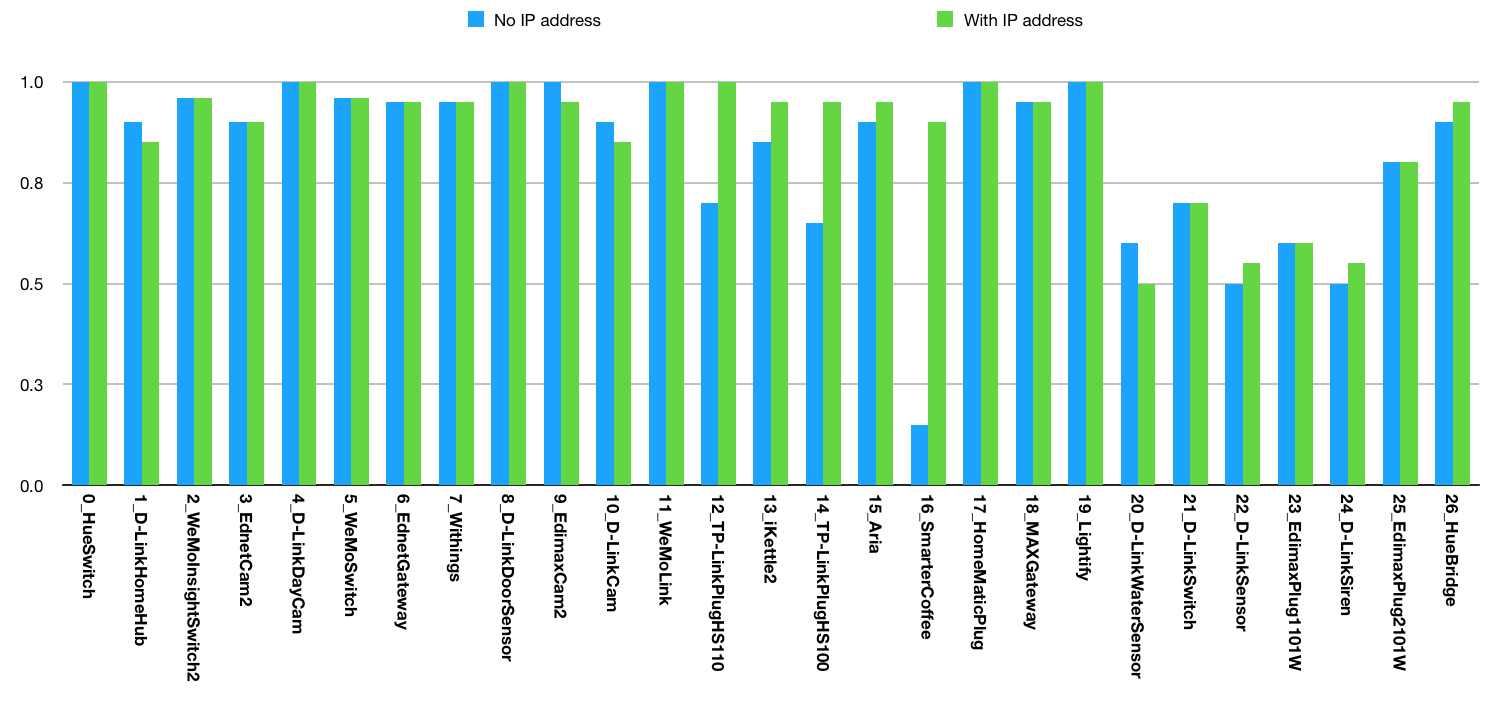
\includegraphics[scale=0.3]{res3}
  \caption{Performance for features with IP addresses and without with IP addresses.}
  \label{fig: res3}
\end{figure}


\section{Conclusion}

From our experiment, we learned that one of the biggest challenge in IoT device identification is to distinguish different device types from the same manufacture because they tend to share similar traffic pattern. In our work, we found that two layers of classifiers (random forest followed by edit distance) can provide better classification accuracy than one layer of classifier (random forest) in this case. Another finding about classifier combination is that a single layer of random forest classifier is capable of providing a satisfying accuracy about 95\% in other cases. This indicates that it’s possible to simplify the classification process by using only one layer of classifier. If the classification result of the first layer shows that this device belongs to a manufacture with many  similar devices, a second layer classifier can be used to further improve accuracy. 

This finding about classifier combination also enables the classification to be performed in real time. Because the second layer classifier, edit distance classifier, can takes a considerable amount of time to run when there are many potential device types. On the other hand, the random forest classifier has a short and stable running time. Separation of the random forest classifier allows the classification to be done in real time.

We also found that it’s possible to improve the classification accuracy for devices from the same manufacture by better feature engineering techniques. Some features are more deterministic than the others, like source and destination IP addresses appeared during device setup. Because other features like packets size, packets number and sequence tend to be similar for those devices. Different IP addresses indicate communications happening with different servers during device setup, which is a potential evidence for different device type. Including such deterministic features can improve the classification accuracy as shown in our experiment result.

Another challenge is the identification of unauthorized devices. In experiments we found that it’s difficult to train a classifier that can balance the accuracy between same device type from different manufactures and different device type from the same manufacture, because those two problems require the classifier to have different decision boundaries. The way we solve this problem is to train classifiers that can classify different device type from the same manufacture, then map the fine-granularity classification result to a general device type using a manually generated list. To classify device from a unseen manufacture, we have to make it being “seen” in training data. In other words, this method requires a traffic dataset with wide coverage for mainstream IoT manufactures. For devices made by manufactures other than those known ones, it should be considered as suspicious and labeled as new device. This requirement for large, wide-coverage dataset leads to another finding of this work that building a large public traffic dataset may be helpful in IoT device type identification study. 

During our experiment setup, we found that capturing traffic is a difficult task because different machines will get slightly different traffic patterns due to network configuration differences and such inconsistent data capture will drop classification accuracy. To train a classifier, large amount of training data is required. It would be very helpful to have a large traffic dataset. However, the non-standard traffic captures settings makes it hard to make use of those datasets because we can’t reproduce comparable captures locally. Considering the lack of device is also a challenge faces by studies on  IoT device identification, if the capture setting and data format can be standardized, it will possible to build a large public traffic dataset that facilitates IoT device identification study.


\section{Future work}

\textbf{More consistency on different setup environments}
During environment setup and traffic capturing, we noticed that the traffic captured under different setup environments may vary. The packets that got captured can vary a lot, and thus the extracted features vary significantly. In such cases, if we train our model with only data captured from one environment, our model might not perform well in another environment because it doesn’t recognize features extracted from setup packets in the new environment. 

We would like our model to be more consistent on different environments. One solution is to set up as many different environments as possible and train our model on data captured from these different environments.

\textbf{Security Enhancement: traffic mimicking} Our demo captures the first N packets when a new MAC address is detected as packets during the setup period. However, attackers might learn about this behavior and try to mimic legit setup traffic for that number of packets or seconds. After it is classified as a legit device, the attacker then starts sending its real setup traffic. Our simple traffic capturer won’t notice this. Thus, we need some capturer that can understand truly when the setup period begins, and not just assume that it begins only when a new MAC address is detected. 

\textbf{Dataset for device type identification} During this project, we spent a lot of time setting up the environment for capturing traffic, and capturing traffic during device setup. We had to reset the devices for each capture, and it is tedious and boring. We hope that there can be some big open datasets for device type identification that includes most common IoT devices, so researchers can focus on improving algorithms rather than environment setup. 





\nocite{*} 
\bibliographystyle{IEEEtranS}
\normalbaselines
\bibliography{References} 


\end{document}

